\documentclass[12pt]{article}
\usepackage{light}

\hidesolutions
%\showsolutions

\newcommand{\edge}[2]{#1\text{---}#2}
\newcommand{\mfigure}[3]{\bigskip\centerline{\resizebox{#1}{#2}{\includegraphics{#3}}}\bigskip}

\begin{document}

\recitation{10}{October 13, 2010}

%%%%%%%%%%%%%%%%%%%%%%%%%%%%%%%%%%%%%%%%%%%%%%%%%%%%%%%%%%%%%%%%%%%%%%%%%%%%%%%

\section*{Analysis of Two Networks}

Two communication networks are shown below.  Complete the table of
properties and be prepared to justify your answers.

\begin{center}
\begin{tabular}{ccc}
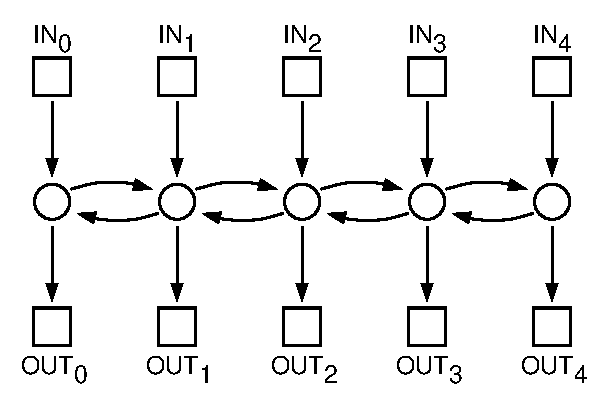
\includegraphics[height=1.5in]{line-nw} & & 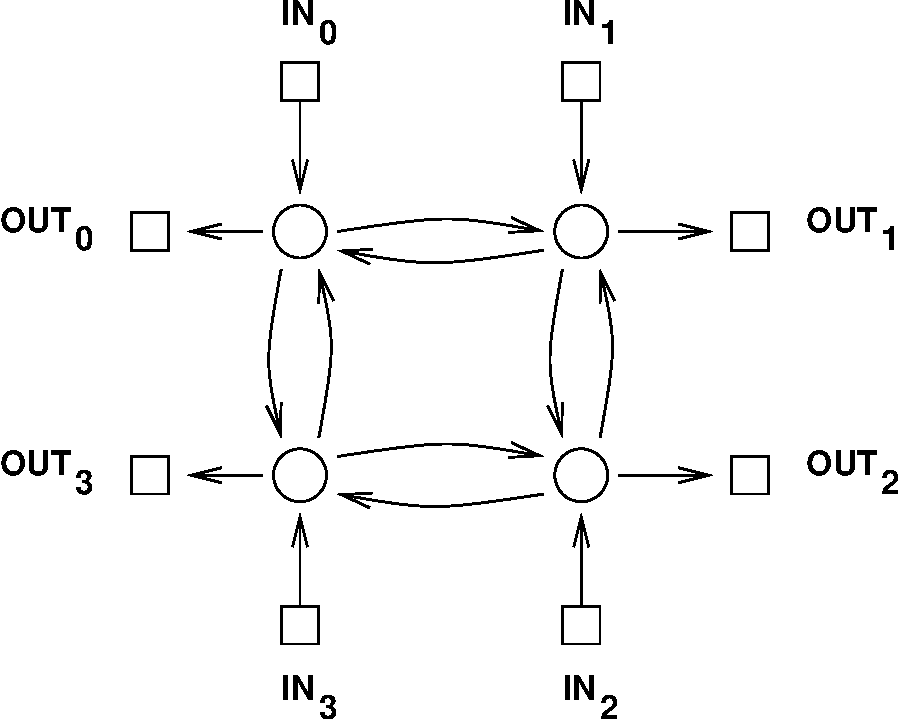
\includegraphics[height=2in]{cycle4} \\
\textbf{5-Path} & \qquad & \textbf{4-Cycle}
\end{tabular}
\end{center}

{\large
\[
\begin{array}{c|c|c|c|c}
\text{network} &
\text{\# switches} &
\text{switch size} &
\text{diameter} &
\text{max congestion} \\ \hline
\text{5-path} &
\insolutions{5} &
\insolutions{3 \times 3} &
\insolutions{6} &
\insolutions{5} \\ \hline
\text{4-cycle} &
\insolutions{4} &
\insolutions{3 \times 3} &
\insolutions{4} &
\insolutions{3}
\end{array}
\]
}

Recall that the \term{diameter} of a communication network is the
number of edges on the shortest path between the input and output
that are farthest apart.  The \term{max congestion} of a network is
the largest number of packets that pass through any switch in the best
solution to the hardest permutation routing problem.
You might imagine that your enemy picks a permutation and then you
pick the path taken by each packet.  (Her goal is to cause congestion,
and yours is to eliminate it.)  Assuming you both do your best, the
max congestion is then equal to the largest number of packets passing
through a single switch.
%
%More formally, the max congestion is the:
%
%\begin{center}
%\begin{tabular}{ll}
%       & maximum over all permutations $\pi$ \\
%of the & minimum over all sets of paths $P_{0, \pi(0)}, \ldots, P_{N-1, \pi(N-1)}$ \\
%of the & maximum over all switches $s$ \\
%of the & number of paths $P_{i, \pi(i)}$ containing switch $s$.
%\end{tabular}
%\end{center}
%
\solution{The congestion of the 5-path is at least 5, because every
path must contain the central switch when $\pi(i) = 4- i$.  The
congestion is at most 5, because there are only 5 paths in total.

The congestion of the 4-cycle is at least 3.  Consider the permutation
routing problem in which each input sends a packet to the diagonally
opposite output: $\pi(0) = 2$, $\pi(1) = 3$, $\pi(2) = 0$, $\pi(3) =
1$.  Packets 0 and 2 must pass through the switches on the upper left
and lower right in order to access the appropriate input and output
terminals.  Packet 1 must pass through one of these switches as well,
so at least three packets pass through either the upper-left switch or
the lower-left switch.

The congestion of the 4-cycle is at most 3.  Suppose we route each
packet by the shortest path and break ties by routing clockwise around
the cycle.  Now consider any particular switch, say the one in the
upper right.  At worst, this switch sees three packets: the one from
input 1, the one destined for output 1, and one passing through from
input 0 to output 2.  By symmetry, every switch sees at most 3 packets.}

%%%%%%%%%%%%%%%%%%%%%%%%%%%%%%%%%%%%%%%%%%%%%%%%%%%%%%%%%%%%%%%%%%%%%%%%%%%%%%%

\instatements{\newpage}

\section*{Routing in a Bene\u{s} Network}

In lecture, we saw that the Bene\u{s} network has a max congestion of
1; that is, every permutation can be routed in such a way that a
single packet passes through each switch.  Let's work through an
example.  A Bene\u{s} network of size $N = 8$ is attached.

\begin{enumerate}
\item Within the Bene\u{s} network of size $N = 8$, there are two
subnetworks of size $N = 4$.  Put boxes around these.  Hereafter,
we'll refer to these as the \textit{upper} and \textit{lower}
subnetworks.

\solution{
\ \\
\mfigure{!}{2in}{benes-decomp}
}

\item Now consider the following permutation routing problem:
%
\begin{align*}
\pi(0) & = 3 & \pi(4) & = 2 \\
\pi(1) & = 1 & \pi(5) & = 0 \\
\pi(2) & = 6 & \pi(6) & = 7 \\
\pi(3) & = 5 & \pi(7) & = 4
\end{align*}
%
Each packet must be routed through either the upper subnetwork or the
lower subnetwork.  Construct a graph with vertices 0, 1, \ldots, 7 and
draw a \textit{dashed} edge between each pair of packets that can not
go through the same subnetwork because a collision would occur in the
second column of switches.

\solution{
\ \\
\mfigure{!}{2in}{rec-const1}
}

\item Add a \textit{solid} edge in your graph between each pair of
packets that can not go through the same subnetwork because a
collision would occur in the next-to-last column of switches.

\solution{
\ \\
\mfigure{!}{2in}{rec-const2}
}

\item Color (i.e., label) the vertices of your graph red and blue so
  that adjacent vertices get different colors.  Why must this be
  possible, regardless of the permutation $\pi$?

\solution{This must be possible, because the dashed edges form a
matching and the solid edges form another matching.  Because of the
result you proved in homework, when you combine the edges, the result
is a bipartite graph, which must be 2-colorable.
%
%This must be possible, because edges in a cycle are
%alternately dashed and solid.  Thus, every cycle has even length,
%which implies that the graph is bipartite or, equivalently,
%2-colorable.

\mfigure{!}{2in}{rec-const3}
}

\item Suppose that red vertices correspond to packets routed through
the upper subnetwork and blue vertices correspond to packets routed
through the lower subnetwork.  On the attached copy of the Bene\u{s}
network, highlight the first and last edge traversed by each packet.

\solution{
\ \\
\mfigure{!}{3in}{rec-benes1}
}

\item All that remains is to route packets through the upper and
lower subnetworks.  One way to do this is by applying the procedure
described above recursively on each subnetwork.  However, since the
remaining problems are small, see if you can complete all the paths 
on your own.

\solution{
\ \\
\mfigure{!}{3in}{rec-benes2}
}

\end{enumerate}

\instatements{\newpage}

\rotatebox{90}{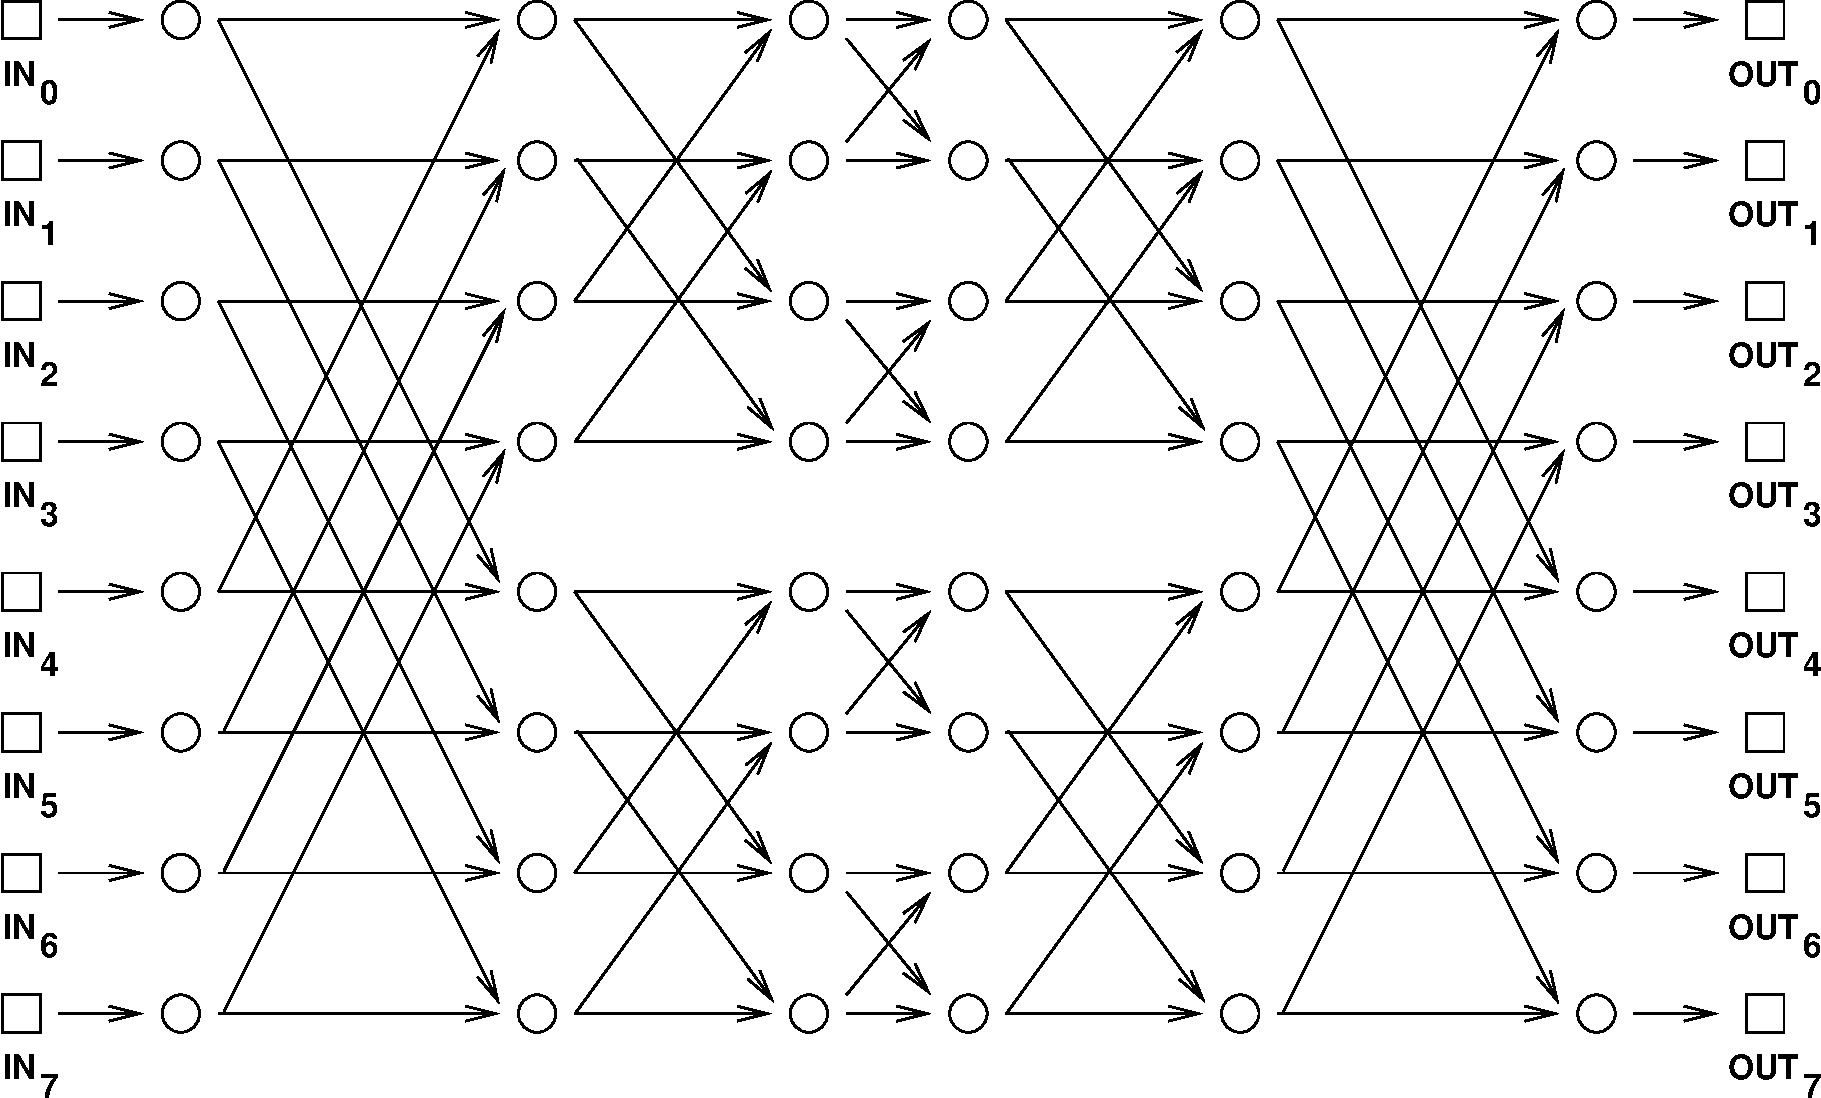
\includegraphics
[width=8.25in]{benes}}

%%%%%%%%%%%%%%%%%%%%%%%%%%%%%%%%%%%%%%%%%%%%%%%%%%%%%%%%%%%%%%%%%%%%%%%%%%%%%%%

\end{document}
